%----------------------------------------------------------------------------------------
%	STEP BY STEP
%----------------------------------------------------------------------------------------

\textit{Ce projet est grandement inspiré d'un sujet proposé par \textit{Hervé SAUER} - enseignant-chercheur retraité de l'Institut d'Optique - en Calcul Scientifique il y a quelques années.}

\section{Introduction}

On se propose dans ce projet de simuler \textbf{l'éclairement} produit par un \textbf{ensemble de sources lumineuses incohérentes} sur un plan en deux dimensions.

\medskip

Ci-dessous une représentation de l'ambiance lumineuse basée sur la modélisation de sources lumineuses à l'aide d'un logiciel spécialisé de conception d'environnement d'éclairage en 3D - DIALux.

\begin{center}
	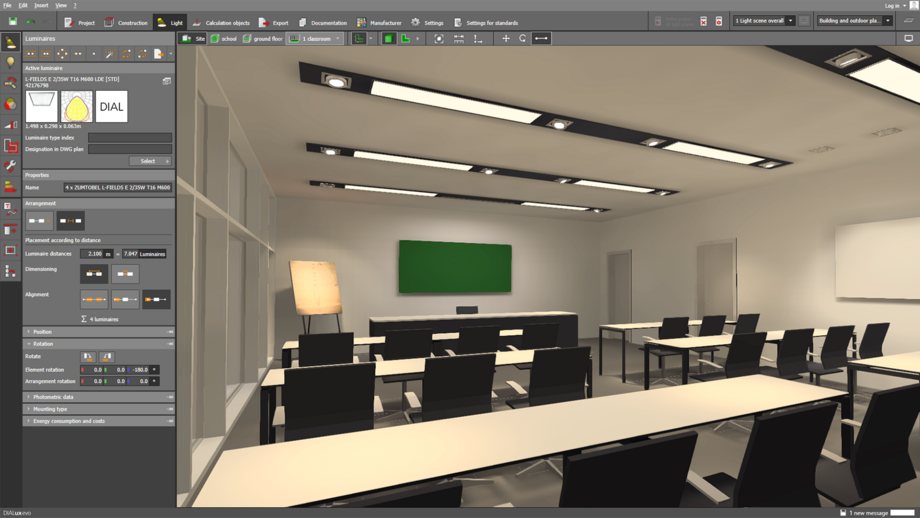
\includegraphics[width=7cm]{ \dirName /images/csm_DIALux-evo_Header_Scene-3-min_d6fe872b15.png}
\end{center}


\section{Objectifs}

\subsection{Modélisation simple}

Dans le cadre de ce projet, on souhaite obtenir une \textbf{cartographie en deux dimensions} d'un ensemble de sources à LEDs positionnées dans un espace en trois dimensions (voir figure \ref{schema}).

On partira d'un modèle simplifié d'une source lumineuse, repérée dans un espace en trois dimensions, dont la directivité de l'intensité sera perpendiculaire au plan de travail considéré et avec une intensité lumineuse donnée (figure \ref{schema}.(a) : l'angle $\theta = -\pi$ dans la figure suivante et un plan horizontal $n_\Pi = [0, 0, 1]$), pour ensuite enrichir le modèle en intégrant la possibilité de réorienter les sources par rapport à la normale du plan considéré (figure \ref{schema}.(b)).

\begin{figure}[h]
	\centering
	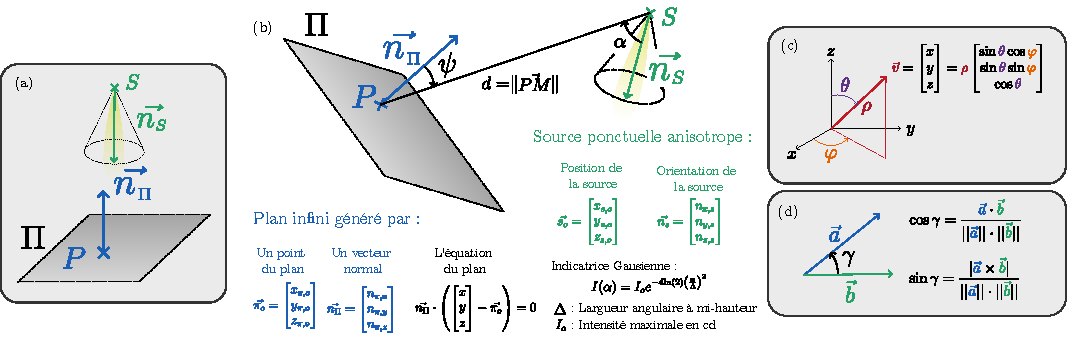
\includegraphics[width=\textwidth]{\dirName /images/ONIP_LED_SCHEMA_UPDATED_V2.pdf}
	\caption{Schéma de principe de la géométrie d'une source positionnée au point $S$ et d'un plan $\Pi$. On représente ici un point $P$ du plan.
	(a) Situation de départ simplifiée avec un plan horizontal et une source dont la direction est perpendiculaire au plan $\Pi$. 
	(b) Situation générale avec une source et un plan orientés de manière arbitraire. L'éclairement sur l'ensemble du plan $\Pi$ peut être déterminé avec les angles non orientés $\psi$ et $\alpha$. $\vec{n_s}$ et $\vec{n_\Pi}$ sont respectivement le vecteur d'orientation de la source et le vecteur normal au plan $\Pi$ dans le système de coordonnées Cartésien $(x, y, z)$. 
	(c) Rappel de transformation d'un système de coordonnées sphérique à un système Cartésien. (utile pour l'orientation de la source selon $(\theta, \varphi)$, voir ci-dessous). 
	(d) Calcul de angle $\gamma$ entre deux vecteurs quelconques $\vec{a}$ et $\vec{b}$.}
	\label{schema}
\end{figure}

Chaque source sera considérée comme indépendante des autres (incohérence) et il sera alors possible de complexifier le système en paramétrant un ensemble N de sources lumineuses et d'en obtenir la cartographie sur un plan donné.

\subsection{Conception de système d'éclairage}

Lorsque l'on conçoit un système d'éclairage, le but le plus souvent recherché est d'avoir un éclairement le plus uniforme et le plus lumineux possible sur une zone donnée en disposant de manière appropriée les sources dont on dispose. 

\medskip

A partir du modèle établi précédemment, il sera alors possible d'optimiser sous contrainte en minimisant la variance ou la valeur absolue de l'écart ou la valeur absolue de l'écart crête à la valeur moyenne de l'éclairement sur la zone considérée avec une contrainte d'éclairement moyen minimum et d'éventuelles contraintes supplémentaires sur le positionnement des sources pour modéliser des limitations ou impératifs mécaniques de placement de celles-ci.

\medskip

\textit{Par exemple, on pourra étudier le placement optimal sur un cercle de diamètre D et d'altitude z0 variables, de N DELs (par exemple, 5 ou 7) de même type (mêmes I0 et mêmes D), en fonction de la directivité des DEL (paramètre D), et de l'éclairement moyen (e.g. 10, 100 voire 1000 lux) souhaités sur un disque de diamètre d (3 ou 4 cm) donné... }


%%%%%%%%%%%%%%%%%%%%%%%
\section{Grandes étapes}

\begin{itemize}
	\item Définir une source lumineuse
	\item Définir un plan de travail
	\item Définir un système comprenant un plan de travail et un ensemble de sources lumineuses
	\item Calculer l'éclairement produit en tout point (discrétisés) du plan de travail par chacune des sources lumineuses
	\item Calculer l'éclairement de l'ensemble des sources et afficher la carte d'éclairement
	\item Calculer la valeur moyenne et l'écart-type de l'éclairement produit sur un plan
\end{itemize}

\medskip

\textit{Afin de simplifier la phase de développement et d'essais de votre application, nous vous suggérons de commencer à réaliser vos modélisations de la façon suivante : }

\begin{description}
	\item[Essai 1] Carte d'éclairement pour une source ponctuelle à une position (x0, y0, z0) - pour différentes valeurs d'angle d'ouverture - direction perpendiculaire par rapport au plan éclairé (cas (a))
	\item[Essai 2] Carte d'éclairement pour une source ponctuelle à une position (x1, y1, z1) différente  - direction perpendiculaire par rapport au plan éclairé (cas (a))
	\item[Essai 3] Carte d'éclairement pour N sources ponctuelles - direction perpendiculaire par rapport au plan éclairé (cas (a))
\end{description}

%%%%%%%%%%%%%%%%%%%%%%%
\section{Modélisation des sources et calcul d'éclairement}

\subsection{Modélisation d'une diode électroluminescente}


Les sources (par exemple des LEDs) seront modélisées de manière approchée (valable si l'on n'est pas trop près du composant) comme des \textbf{sources ponctuelles}. Ces sources ont un \textbf{diagramme de rayonnement} possédant une \textbf{symétrie de révolution} autour d'un axe orienté. 

\medskip

L'indicatrice de rayonnement pourra être considérée comme gaussienne, et caractérisée par son intensité visuelle vers l'avant sur l'axe $I_0$ (en candela) et sa largeur totale à mi-hauteur $\Delta$.

Cette indicatrice peut-être modélisée par l'équation suivante : $$I(\alpha) = I_0 \cdot \exp(-(4 \cdot \ln(2)) \cdot (\alpha/\Delta)^2)$$

où $\alpha$ est l'angle entre la direction d'émission et l'axe de la source ($\alpha \in [0^{\circ}, 180^{\circ}]$). 

\medskip

%%%%%%%%%%%%%%%%%%%%%%%
\subsection{Positionnement d'une source}

Le positionnement de la source dans l'espace sera caractérisé par ses coordonnées $(x, y, z)$ et l'orientation de son axe de symétrie (\textit{i.e.} là où sont intensité est maximale) par deux angles ($\theta$ et $\varphi$) dans le système de coordonnée sphérique centrée sur la source. 
	
\medskip

%%%%%%%%%%%%%%%%%%%%%%%
\subsection{Eclairement / Formule de Bouguer}

L'éclairement fourni par une source ponctuelle en un point P de l'espace séparé d'une distance $d$ et d'une inclinaison de $\psi$ par rapport à la direction de la source ponctuelle, est données par la relation photométrique suivante : 

$$E = \frac{I(\alpha) \cdot \cos(\psi)}{d^2}$$


%%%%%%%%%%%%%%%%%%%%%%%

L'éclairement produit par N sources (incohérentes) est la somme des éclairements produits par chaque source.

